\documentclass[answers]{exam}
% 'texPreamble' contains formatting and macros. 
% https://github.com/pwesterbaan/scripts/tree/master/texmf/tex/latex/local
\usepackage{texPreamble}
\hypersetup{hidelinks}
\usepackage{relsize}
\usepackage{tkz-euclide}
\usepackage[titles]{tocloft}
\renewcommand{\cftsecleader}{\cftdotfill{\cftdotsep}}
\usetkzobj{all}
%% Externalize graphics and save in ./images/ folder
%% pdflatex -shell-escape <tex file>
%% The document can be compiled with the two following
%% lines commented out, but will recompile all figures
%% each time.
\usetikzlibrary{external}
\tikzexternalize[prefix=images/]
%% 
\usepackage{tabularx}
\extraheadheight{0.25in}
\extrafootheight{1.0in}
\extrawidth{1in}
% ----------------------------------------------------------------
\makeatletter
\title{Math 1070 Class notes\\[0.25\baselineskip]Spring 2020}
\author{\thefname\ \thelname}

\pagestyle{headandfoot}

%\firstpageheader{\@title\\\@date}{}{Math 1070}
%\firstpageheadrule

\newcommand*{\currentname}{\@currentlabelname}

\runningfootrule
\runningfooter{\parbox{0.45\linewidth}{\currentname}}{\thepage}{\@title}
\makeatother

\begin{document}
  %% Title
  \pagenumbering{roman}
  \vspace*{\stretch{1}}
  \begin{center}
    \makeatletter
    {\huge
    \@title}\\[\baselineskip]
    \@author\\[\baselineskip]
    Last updated:
    \@date\\
    \makeatother
  \end{center}
  \vspace*{\stretch{1}}
  \thispagestyle{empty}
  \pagebreak
  \pagestyle{headandfoot}

  \renewcommand{\contentsname}{Table Of Contents}
  \renewcommand\thesection{}
  \tableofcontents
  \newpage
  
  \makeatletter
  \firstpageheader{}{}{}
  \firstpagefooter{\parbox{0.45\linewidth}{\currentname}}{\thepage}{\@title}
  \firstpagefootrule
  \makeatother
  \pagenumbering{arabic}
  \setcounter{page}{1}
  %% everything else
  \relscale{1.4}

\documentclass[answers]{exam}
\usepackage{texPreamble}
\usepackage{relsize}
\usepackage{tabularx}
\extraheadheight{0.25in}
\extrafootheight{1.0in}
\extrawidth{1in}
% ----------------------------------------------------------------
\firstpagefootrule
\runningfootrule
\begin{document}
%\relscale{1.4} %TODO
\section{MATH 1040 Review}
  For the following functions, find their derivatives:
  \begin{tasks}[label=\hspace*{0pt},after-item-skip=\stretch{0.5}](2)
    \task $y=\sqrt[7]{x^3}-\pi e^x+x^e+3e\inv[x]$
    \task $f(x)=\parens{\frac{1-\sin(x)}{1+\cos(x)}}$
    \task $g(x)=\parens{\frac{x^2+3x+1}{e^x}}$
    \task $h(y)=-5\cot\parens{3e^{4y}}+e^\pi$
  \end{tasks}
  \vspace*{\stretch{0.5}}
  Find $f''(x)$ for $f(x)=\tan(x)$
  \vspace*{\stretch{1}}
  \pagebreak
  
  Find the equation of the line tangent to $\ell(x)=x\sqrt{5-x^2}$ at the point $(1,2)$.
  \vspace*{\stretch{1}}
  
  Where is the tangent line of $u=\dfrac{1}{\sqrt x}$ parallel to the line $y=-4x-3$?
  \vspace*{\stretch{1}}
  \pagebreak

  %% 01/14/19
  \noindent
  \textbf{Note:} Limits will be on Test 1 and the final exam.
  \begin{ex*}~

  Using the graph below, evaluate each limit:
  \end{ex*}
  
  \begin{minipage}{0.275\linewidth}
    \begin{tikzpicture}
      \begin{axis}[
        axis lines=center,
        axis line style={->},
        xmin=-1.5, xmax=2.25, 
        ymin=-0.5, ymax=1.5,
        xtick={-6,-5,...,6},
        ytick={-6,-5,...,6},
        ticklabel style={font=\footnotesize,inner sep=0.5pt,fill=white,opacity=1.0, text opacity=1},
        height=0.95*2.0in, width=0.75*3.75in,
        xlabel=$x$, xlabel style={at={(ticklabel* cs:1)},anchor=north west},
        ylabel=$y$, ylabel style={at={(ticklabel* cs:1)},anchor=south west},
        every axis plot/.append style={line width=0.95pt}
        ]
        \addplot[-] expression[domain=-1:1, blue]{x^2};
        \node[anchor=south west] at(axis cs: 0.85,1.05) {$y=f(x)$};
        \addplot[-] expression[domain=1:2, blue]{0};
        \addplot[soldot] coordinates{(-1,1)(0,1)(1,0)(2,0)};
        \addplot[holdot] coordinates{(0,0)(1,1)};
      \end{axis}
    \end{tikzpicture}
  \end{minipage}%
  \begin{minipage}{0.725\linewidth}
    \begin{tasks}[label=~, after-item-skip=20pt](3)
      \task $\ds\lim_{x\to -1^+} f(x)$
      \task* $\ds\lim_{x\to 2^-} f(x)$
      \task $\ds\lim_{x\to 0^-} f(x)$
      \task $\ds\lim_{x\to 0^+} f(x)$
      \task $\ds\lim_{x\to 0} f(x)$
      \task $\ds\lim_{x\to 1^-} f(x)$
      \task $\ds\lim_{x\to 1^+} f(x)$
      \task $\ds\lim_{x\to 1} f(x)$
    \end{tasks}
  \end{minipage}
  
  \vspace*{15pt}
  State the intervals of continuity on $[-1,2]$.
  \vspace*{\stretch{0.5}}
  \begin{ex*}
    Algebraically, evaluate the following limits
  \end{ex*}
  \begin{tasks}[label=\hspace*{0pt}, after-item-skip=\stretch{1}](2)
    \task $\ds\lim_{x\to 0}\parens{\sin^2 x+\sec x}$
    \task $\ds\lim_{y\to 0}\frac{5y^3+8y^2}{3y^4-16y^2}$
  \end{tasks}
  \vspace*{\stretch{1}}
  \pagebreak
  
  \begin{tasks}[label=\hspace*{0pt}, after-item-skip=\stretch{1}](2)
    \task $\ds\lim_{x\to \frac{1}{2}^-} \frac{4x-2}{\abs{2x^3-x^2}}$
    \task $\ds\lim_{x\to 0} \frac{1-\cos x}{\cos^2 x-3\cos x+2}$
    \task $\ds\lim_{x\to 0} \frac{x}{\sqrt{5x+1}-1}$
    \task $\ds\lim_{x\to 0} \frac{e^{4x}-1}{e^{x}-1}$
    \task $\ds\lim_{x\to 0} \frac{\sin(x)}{x}$
    \task $\ds\lim_{x\to 0} \frac{\tan(3x)}{5x}$
  \end{tasks}
  \vspace*{\stretch{1}}
  \pagebreak
  
  \begin{tasks}[label=\hspace*{0pt}, after-item-skip=\stretch{1}](2)
    \task $\ds\lim_{x\to \infty} \frac{4x^3+1}{2x^3+\sqrt{16x^6+1}}$
    \task $\ds\lim_{x\to -\infty} \frac{4x^3+1}{2x^3+\sqrt{16x^6+1}}$
    \task $\ds\lim_{x\to -\infty} \parens{x+\sqrt{x^2+2x}}$
  \end{tasks}
  \vspace*{\stretch{1}}
  \pagebreak
  
  \begin{tasks}[label=\hspace*{0pt}, after-item-skip=\stretch{1}](2)
    \task $\ds\lim_{t\to -2^-} \frac{t^3-5t^2+6t}{t^4-4t^2}$
    \task $\ds\lim_{t\to -2^+} \frac{t^3-5t^2+6t}{t^4-4t^2}$
    \task $\ds\lim_{x\to -\infty} \frac{3x+7}{x^2-4}$
  \end{tasks}
  \vspace*{\stretch{1}}
  \pagebreak
  
  Find the equation of the slant (oblique) asymptote of $\ds f(x)=\frac{3x^5+x^4+2x^2+1}{x^4+3}$.
  \pagebreak
  
  Find $k$ such that $f(x)$ is continuous at $x=1$:
    $$f(x)=\begin{cases}
      k\,\tan\parens{\frac{\pi x}{3}},& x\geq 1\\
      x-2,& x<1
    \end{cases}$$
  \vspace{\stretch{1}}
  
  Find $c$ such that $f(x)$ is continuous:
    $$f(x)=\begin{cases}
      \dfrac{\sin^2 3x}{x^2},& x\neq 0\\
      c,& x=0
    \end{cases}$$
  \vspace*{\stretch{1}}
  \pagebreak 
  
\textbf{$\delta \textnormal{ --- } \eps$ proofs:}

  \begin{center}
    \begin{tikzpicture}[scale=0.825]
      \begin{groupplot}[
        group style={group size=3 by 1},
        axis lines=center,
        axis line style={->},
        xmin=0, xmax=4,
        ymin=0, ymax=4,
        enlargelimits={abs=0.65},
        ticklabel style={font=\large, inner sep=0.75pt,fill=white},
	      every axis plot/.append style={line width=0.95pt}
        ]
        \nextgroupplot[xtick={2.675},ytick={2.9429},
          xticklabels={$a$},yticklabels={$L$},]
          \addplot[-] expression[domain=1.575:3.865, blue] {cot(deg(x-pi/3))+3)};
          \draw[dashed, line width=0.75pt] (axis cs: 0,2.9429) -- (axis cs: 2.675,2.9429) -- (axis cs:2.675,0);
        \nextgroupplot [xtick={2.675},
          ytick={1.7853,2.9429,3.9658},
          xticklabels={$a$},yticklabels={$L-\eps$,$L$,$L+\eps$},]
          \fill[fill=ClemsonPurple, opacity=0.25] (axis cs:0,1.7853) rectangle ++(6,2.1805);
          \addplot[-] expression[domain=1.575:3.865, blue] {cot(deg(x-pi/3))+3)};
          \draw[dashed, line width=0.5pt] (axis cs: 0,1.7853) -- (axis cs: 6,1.7853);
          \draw[dashed, line width=0.5pt] (axis cs: 0,3.9658) -- (axis cs: 6,3.9658);
          \draw[dashed, line width=0.75pt] (axis cs: 0,2.9429) -- (axis cs: 2.675,2.9429) -- (axis cs:2.675,0);
        \nextgroupplot[xtick={1.85,2.675,3.5},ytick={1.7853,2.9429,3.9658},
          xticklabels={$a-\delta$,$a$,$a+\delta$},
          yticklabels={$L-\eps$,$L$,$L+\eps$},]
          \fill[fill=ClemsonOrange, opacity=0.25] (axis cs:1.85,0) rectangle ++(1.65,6);
          \fill[fill=ClemsonPurple, opacity=0.25] (axis cs:0,1.7853) rectangle ++(6,2.1805);
          \addplot[-] expression[domain=1.575:3.865, blue] {cot(deg(x-pi/3))+3)};
          \draw[dashed, line width=0.5pt] (axis cs: 1.85,0) -- (axis cs: 1.85,6);
          \draw[dashed, line width=0.5pt] (axis cs: 3.5,0) -- (axis cs: 3.5,6);
          \draw[dashed, line width=0.5pt] (axis cs: 0,1.7853) -- (axis cs: 6,1.7853);
          \draw[dashed, line width=0.5pt] (axis cs: 0,3.9658) -- (axis cs: 6,3.9658);
          \draw[dashed, line width=0.75pt] (axis cs: 0,2.9429) -- (axis cs: 2.675,2.9429) -- (axis cs:2.675,0);
      \end{groupplot}
    \end{tikzpicture}
  \end{center}


\def\scale{0.85}
  \begin{ex*}
    Use the graph of $f$ below to find a number $\delta$ such that if $0<\abs{x-2.25}<\delta$ then $\abs{f(x)-2.159}<1$.
  \end{ex*}
\begin{flushright}
  \begin{tikzpicture}[scale=\scale]
    \begin{axis}[
      axis lines=center,
      axis line style={->},
      xmin=-0.5, xmax=3.25,
      ymin=-0.5, ymax=4,
      xtick={1.409,2.25,2.991},
      xticklabels={1.409,2.250,2.991},
      ytick={1.159,2.159,3.159},
      yticklabels={1.159,2.159,3.159},
      xticklabel style={font=\large, rotate=-25, yshift=5pt},
      yticklabel style={font=\large},
      every axis plot/.append style={line width=0.95pt}
      ]
      \addplot[-] expression[domain=-1.25:5, blue] {5/(1+3^(2.5-x))};
      \draw[dashed] (axis cs: 0,1.159) -- (axis cs: 1.409,1.159) -- (axis cs: 1.409,0);
      \draw[dashed] (axis cs: 0,3.159) -- (axis cs: 2.991,3.159) -- (axis cs: 2.991,0);
      \draw[loosely dotted, line width=1.25pt] (axis cs: 0,2.159) -- (axis cs: 2.25,2.159) -- (axis cs: 2.25,0);
    \end{axis}
  \end{tikzpicture}
\end{flushright}
\begin{ex*}
  Use the graph of $g(x)=\sqrt x+1$ to help find a number $\delta$ such that if $\abs{x-4}<\delta$ then $\ds\abs{\parens{\sqrt x+1}-3}<\frac{1}{2}$.
\end{ex*}
  \begin{tikzpicture}[scale=\scale]
    \begin{axis}[
      axis lines=center,
      axis line style={->},
      xmin=-0.25, xmax=7.25,
      ymin=-0.25, ymax=4.5,
      xtick={2.25,4,6.25},
      xticklabels={$x_1$,4,$x_2$},
      ytick={2.5,3,3.5},
      ticklabel style={font=\large, inner sep=0.75pt},
      every axis plot/.append style={line width=0.95pt}
      ]
      \addplot[-] expression[blue, samples at={0,0.05,...,7.25}] {sqrt(x)+1};
      \draw[dashed] (axis cs: 0,2.5) -- (axis cs: 2.25,2.5) -- (axis cs: 2.25,0);
      \draw[dashed] (axis cs: 0,3.5) -- (axis cs: 6.25,3.5) -- (axis cs: 6.25,0);
      \draw[loosely dotted, line width=1.25pt] (axis cs: 0,3) -- (axis cs: 4,3) -- (axis cs: 4,0);
    \end{axis}
  \end{tikzpicture}
\pagebreak

\begin{ex*}
Algebraically, prove the following limits:
\end{ex*}
\begin{enumerate}[itemsep=\stretch{1}, label=\hspace*{0pt}]
  \item $\ds\lim_{x\to 3}\parens{10-3x}=1$
  \item $\ds\lim_{x\to 14}\parens{2-\frac{2}{7}x}=-2$
  \item $\ds\lim_{x\to 3}\frac{x^2+x-12}{x-3}=7$
\end{enumerate}
\vfill
\pagebreak

\textbf{Rates of change}
\begin{ex*}
  Find the average rate of change of $f(x)=3x^2-4x$ over the interval $\sbrkt{-1,4}$ and the instantaneous rate of change at $x=3$.
\end{ex*}
\vfill
\textbf{Limit definition of the derivative}
Recall the following definition:
  $$f'(x)=\lim_{h \to 0}\frac{f(x+h)-f(x)}{h}$$
\begin{ex*}
  Use the limit definition of the derivative to find $f'(x)$ when $f(x)=-\frac{1}{x^2}$ and then evaluate $f'(3)$.
\end{ex*}
\vfill
\pagebreak

\begin{ex*}
  Use the limit definition of the derivative to find $f'(x)$ when $f(x)=\frac{1-x}{2x}$.
\end{ex*}
\vfill

\noindent
\begin{minipage}{0.5\linewidth}
  \begin{center}
    \begin{tabularx}{0.9\linewidth}{@{}YY@{}}\toprule
      Function& Derivative\\\midrule
      Increasing&\\
      Decreasing&\\
      Max/Min&\\
      Inflection point&\\
      Constant&\\
      Linear&\\
      Quadratic\\\bottomrule
    \end{tabularx}
  \end{center}
\end{minipage}%
\begin{minipage}{0.5\linewidth}
  A function is not differentiable wherever it has a
  \begin{enumerate}[itemsep=20pt]
    \item \fillin[][\linewidth]
    \item \fillin[][\linewidth]
    \item \fillin[][\linewidth]
  \end{enumerate}
\end{minipage}%
\pagebreak

\textbf{The Chain Rule and Product Rule}
\begin{ex*}
  Find the derivatives of the following functions
\end{ex*}
\begin{tasks}[after-item-skip=\stretch{1}, label=\hspace*{0pt}](2)
  \task $y=\cos\parens{2x^5+7x}$
  \task $p(x)=\sqrt2x+\sqrt{3x}$
  \task $y=x^{2e}-e^{\frac{3x-2}{x^2-3x}}$
  \task $y=f\parens{\sqrt[3]{g(4x^3)}}$
\end{tasks}
\vfill
\pagebreak

\begin{tasks}[after-item-skip=\stretch{1}, label=\hspace*{0pt}](2)
  \task $\dfrac{d}{dx}\sbrkt{\frac{f(x)-3g(x)}{2}}$
  \task $\dfrac{d}{dx}\sbrkt{\frac{x\sbrkt{g(x)}^2}{h(x)}}$
  \task $h(\theta)=\sqrt[3]{-\theta+\cot(9+2\theta)}$
  \task $y(\theta)=\tan^2\parens{\cot(3\theta)}$
\end{tasks}
\vfill
\pagebreak

\begin{tasks}[after-item-skip=\stretch{1}, label=\hspace*{0pt}](2)
  \task $y=3x^2\parens{e\inv[x]+2}^4\tan\parens{3x+2}$
  \task $h(x)=\frac{-1}{2\,\sqrt[5]{\csc^2(4x)}}$
\end{tasks}
\vfill 

\begin{ex*}
  Let $f(1)=3, f'(1)=4, g(1)=2, g'(1)=6, g(3)=5$ and $g'(3)=2$. 
  
  Now, let $H(x)=\parens{g\circ f})(x)=g\parens{f(x)}$ and find $H'(1)$.
\end{ex*}
\vfill 

\begin{ex*}
  Find $\dfrac{d^2}{d\theta^2}\sbrkt{\sin^2(3\theta)}$.
\end{ex*}
\vfill 
\pagebreak 

  %TODO Comment out relsize!
\end{document}

\documentclass[../mathNotesPreamble]{subfiles}
\begin{document}
%\relscale{1.4}
\section{JIT 13.1: Solving Linear Equations Involving Derivatives}
Recall that for a function $f(x)$, we can denote the derivative as $\dfrac{df}{dx}$. %In Briggs 3.8, when we do implicit differentiation, we must be able to solve equations for $\dfrac{df}{dx}$
\begin{ex*}
  Solve the following for $\dfrac{dy}{dx}$:
\end{ex*}
\begin{tasks}[after-item-skip=\stretch{1}, label=~](2)
  \task $2+3\dfrac{dy}{dx}=1$
  \task $2x+3y'=3x-5y'$
  \task $x+2y\dfrac{dy}{dx}=-\dfrac{dy}{dx}+y$
  \task $5xy+4\dfrac{dy}{dx}=3x^2-2xy^2\dfrac{dy}{dx}$
\end{tasks}
\vfill
\pagebreak

\end{document}

\documentclass[answers]{exam}
\usepackage{texPreamble}
\usepackage{relsize}
\usepackage{tabularx}
\extraheadheight{0.25in}
\extrafootheight{1.0in}
\extrawidth{1in}
% ----------------------------------------------------------------
\firstpagefootrule
\runningfootrule
\begin{document}
%\relscale{1.4}

\section{3.8: Implicit Differentiation}
Up until now, we have only taken the derivatives of \textit{explicitly} defined functions (functions defined in terms of only $x$). 

\noindent
An \textit{implicitly} defined function will be written in terms of both $x$ and $y$:
  $$x^2+y^2=25$$
\begin{center}
  \begin{tikzpicture}
    \begin{groupplot}[
      group style={group size=2 by 1},
      axis equal,
      axis lines=center,
      axis line style={->},
      ymin=-6.5, ymax=6.5,
      xtick={-5,5},
      ytick={-5,5},
      ticklabel style={font=\large, inner sep=0.75pt,fill=white},
      every axis plot/.append style={line width=0.95pt}, 
      samples=251, domain=-5:5,
      ]
      \nextgroupplot
        \addplot[-] expression[black]{sqrt(25-x^2)} node at (4.45,5.8) {$x^2+y^2=25$};
        \addplot[-] expression[black]{-sqrt(25-x^2)};
      \nextgroupplot
        \addplot[-] expression[ClemsonPurple]{sqrt(25-x^2)} node[black] at (4.1,5.8) {$y=\sqrt{25-x^2}$};
        \addplot[-] expression[ClemsonOrange]{-sqrt(25-x^2)} node[black] at (4.1,-5.5) {$y=-\sqrt{25-x^2}$};
    \end{groupplot}
  \end{tikzpicture}
\vfill 
  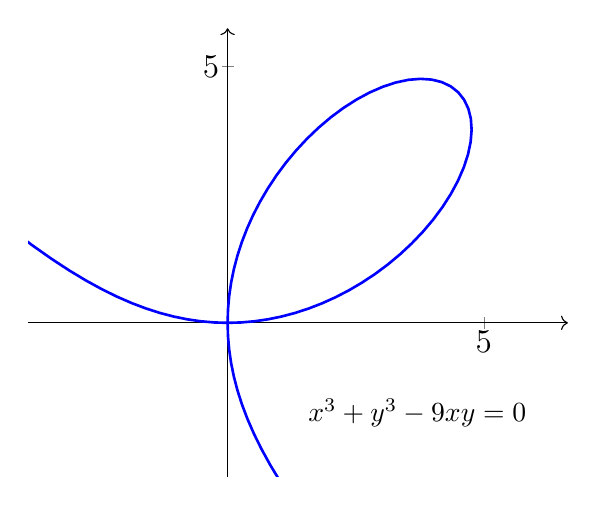
\begin{tikzpicture}
    \begin{axis}[
      axis equal,
      axis lines=center,
      axis line style={->},
      xmin=-3, xmax=5.75,
      ymin=-3, ymax=5.75,
      xtick={-5,5},
      ytick={-5,5},
      ticklabel style={font=\large, inner sep=0.75pt,fill=white},
      ]
      \draw[samples=100,domain=125:-40, line width=0.95pt, blue] plot(\x:{9*sin(\x)*cos(\x)/(sin(\x)^3+cos(\x)^3)}) node[black] at (3.7,-1.75) {$x^3+y^3-9xy=0$};
    \end{axis}
  \end{tikzpicture}
\vfill 
\end{center}
\pagebreak

\begin{center}\fbox{\parbox{0.7\linewidth}{

\textbf{Implicit Differentiation:}
  \begin{enumerate}
    \item Differentiate both sides of the equation with respect to $x$, treating $y$ as a differentiable function of $x$.
    \item Collect the terms with $\sfrac{dy}{dx}$ on one side of the equation.
    \item Solve for $\sfrac{dy}{dx}$.
  \end{enumerate}
}}\end{center}

\begin{ex*}
  Find the derivatives of the following by rewriting each function explicitly before taking the derivative, and by using implicit differentiation. Compare the results.
\end{ex*}

\begin{enumerate}[label=, itemsep=\stretch{1}]
  \item $y^2=x$
  \item $\sqrt x+\sqrt y=4$
\end{enumerate}
\vfill 
\pagebreak
\begin{ex*}
  Find the derivatives of the following equations:
\end{ex*}

\begin{tasks}[after-item-skip=\stretch{1}, label=~](2)
  \task $x^2+y^2=25$
  \task $x^3+y^3-9xy=0$
  \task $2y=x^2+\sin y$
  \task $x^2y^2+x\sin y=4$
  \task $y^5+x^2y^3=1+x^4y$
  \task $1+x=\sin\parens{xy^2}$
\end{tasks}
\vfill
\pagebreak

\begin{ex*}
  Find the derivatives of the following equations:
\end{ex*}
\begin{tasks}[after-item-skip=\stretch{1}, label=~](2)
  \task $x^3-xy+y^3=1$
  \task $xe^y=x-y$
  \task $\dfrac{1}{x}+\dfrac{1}{y}=1$
  \task $x^2-2x^3y^4+y^2=30y$
  \task $\tan(xy)=x+y$
  \task $x^2=\dfrac{x-y}{x+y}$
\end{tasks}
\vfill
\pagebreak

\begin{ex*}
  Find the second derivative implicitly for the following equations:
\end{ex*}
\begin{tasks}[after-item-skip=\stretch{1}, label=~](1)
  \task $y^2-2x=1-2y$
  \task $xy=\cot(xy)$
  \task $x^3+y^3=1$
  \task $x=e^y$
\end{tasks}
\vfill
\pagebreak

\begin{ex*}
  Find the equation of all lines tangent to the curve $x+y^3-y=1$ at $x=1$.
\end{ex*}
\vfill
%% This royal PITA needs to be compiled using 
%% shell-escape since it uses gnuplot
%%%%% pdflatex -shell-escape impFunc.tex %%%%%
\includegraphics[width=0.4\linewidth]{impFunc1}

\begin{ex*}
  Find the equation of the tangent line and normal line for $\parens{x^2+y^2-2x}^2=2\parens{x^2+y^2}$ at $(x,y)=(2,2)$.  
\end{ex*}
\vfill
\includegraphics[width=0.4\linewidth]{impFunc2}

\pagebreak

\end{document}

\input{briggs3_09}
\documentclass[../mathNotesPreamble]{subfiles}
\begin{document}
\tikzset{custNode/.style={color=black,inner sep=0.5pt,fill=none,opacity=1.0, text opacity=1}}
\tikzset{dLine/.style={mark=none, dashed, opacity=1.0, blue!85, line width=0.5pt}}
%\relscale{1.4}
\section{JIT 9.1: Definition of $\arcsin x$, the Inverse Sine Function}
  Recall that a function has an inverse if it is 1-to-1 (e.g. it passes the horizontal line test).
  \begin{center}
    \begin{tikzpicture}
      \begin{groupplot}[
        group style={group size=3 by 1, horizontal sep=1cm},
        width=0.36\linewidth,
        axis lines=center,
        axis line style={->},
        ticklabel style={font=\footnotesize,inner sep=0.5pt,fill=white,opacity=1.0, text opacity=1},
        xlabel=$x$, xlabel style={at={(ticklabel* cs:1)},anchor=north west},
        ylabel=$y$, ylabel style={at={(ticklabel* cs:1)},anchor=south west},
        every axis plot/.append style={line width=0.95pt, color=blue}
        ]
        \nextgroupplot[
          xmin=-4.25, xmax=6.25,
          ymin=-4.25, ymax=6.25,
          xmajorticks=false,
          ymajorticks=false,
          every axis plot/.append style={samples=100},
          ]
          \addplot[dashed] expression[domain=-4.25:6.25, black]{x};
          \addplot[->] expression[domain=-4.25:ln(6.25), ClemsonPurple] {e^x} node[custNode, below right, pos=1] {$a^x$};
          \addplot[->] expression[domain=exp(-4.25):6.25, ClemsonOrange] {ln(x)} node[custNode, above left, pos=1] {$\log_a(x)$};
        \nextgroupplot[
          xmin=-0.5, xmax=3.25,
          ymin=-0.5, ymax=3.25,
          xmajorticks=false,
          ymajorticks=false,
          every axis plot/.append style={samples=500},
          ]
          \addplot[dashed] expression[domain=-0.5:3.25, black]{x};
          \addplot[dashed] expression[domain=-0.5:0, ClemsonPurple]{x^2};
          \addplot[->] expression[domain=0:sqrt(3.25), ClemsonPurple]{x^2} node[custNode, below right, pos=1] {$x^2$};
          \addplot[->] expression[domain=0:3.25, ClemsonOrange]{sqrt(x)} node[custNode, above left, pos=1] {$\sqrt x$};
        \nextgroupplot[
          xmin=-(pi/2+0.5), xmax=(pi/2+0.775),
          ymin=-(pi/2+0.5), ymax=(pi/2+0.65),
          xmajorticks=false,
          ymajorticks=false,
          every axis plot/.append style={samples=100},
          ]
          \addplot[dashed] expression[domain=-(pi/2+0.5):(pi/2+0.775), black]{x};
          \addplot[dashed] expression[domain=-pi/2-0.5:-pi/2, ClemsonPurple]{sin(x*180/pi)};
          \addplot[dashed] expression[domain=pi/2:pi/2+0.775, ClemsonPurple]{sin(x*180/pi)};
          \addplot[-] expression[domain=-pi/2:pi/2, ClemsonPurple]{sin(x*180/pi)} node[custNode, below right, pos=0.85] {$\sin(x)$};
          \addplot[-] expression[domain=-1:1, ClemsonOrange]{asin(x)*pi/180} node[custNode, above, pos=1, xshift=-5pt] {$\arcsin(x)$};
      \end{groupplot}
    \end{tikzpicture}
    
    Notice that $x^2$ and $\sin(x)$ are on restricted domains.
  \end{center}

Without restriction on its domain, $\sin(x)$ is NOT 1-to-1:
\begin{center}
  \begin{tikzpicture}
    \begin{axis}[
      axis lines=center,
      axis line style={->},
      xmin=-7, xmax=7,
      ymin=-1.25, ymax=1.25,
      xtick={-6.28318, -4.7123889, ..., 6.28318},
      xticklabels={$-2\pi$, $-\frac{3\pi}{2}$,$-\pi$, $-\frac{\pi}{2}$, ,
         $\frac{\pi}{2}$,$\pi$, $\frac{3\pi}{2}$, $2\pi$},
      height=1.75in, width=0.9\linewidth,
      ticklabel style={font=\small, inner sep=0.75pt,fill=white},
      xlabel=$x$, xlabel style={at={(ticklabel* cs:1)},anchor=north west},
      ylabel=$y$, ylabel style={at={(ticklabel* cs:1)},anchor=south west},
      every axis plot/.append style={line width=0.95pt, color=blue}
      ]
      \addplot[domain=-6.28:6.28, ClemsonPurple, samples=101] {sin(deg(x))} node[custNode, pos=0.7, above right] {$\sin(x)$};
    \end{axis}
  \end{tikzpicture}
\end{center}

The range of $\sin(x)$ is $[-1,1]$ and all of these values are attained on a restricted domain of $\sbrkt{\nicefrac{-\pi}{2},\nicefrac{\pi}{2}}$:

\begin{center}
  \begin{tikzpicture}
    \begin{groupplot}[
      group style={group size=2 by 1, horizontal sep=4cm},
      axis lines=center,
      axis line style={->},
      xmin=-(pi/2+0.95), xmax=pi/2+0.95,
      ymin=-(pi/2+0.95), ymax=pi/2+0.95,
      width=0.4\linewidth,
      ticklabel style={font=\small, inner sep=0.75pt,fill=white},
      xlabel=$x$, xlabel style={at={(ticklabel* cs:1)},anchor=north west},
      ylabel=$y$, ylabel style={at={(ticklabel* cs:1)},anchor=south west},
      every axis plot/.append style={line width=0.95pt, color=blue, samples=100}      
      ]
      \nextgroupplot[
        xtick={-1.570796327,1.570796327},
        ytick={-1,1},
        xticklabels={$-\frac{\pi}{2}$,$\frac{\pi}{2}$},
        ]
        \addplot[-] expression[domain=-pi/2:pi/2, ClemsonPurple]{sin(x*180/pi)};
        \node[custNode] at (-pi/2,1) {$\sin(x)$};
        \addplot[soldot, black] coordinates{(-pi/2,-1)} node[custNode, below, xshift=5pt, yshift=-4pt] {$\parens{\frac{-\pi}{2},-1}$};
        \addplot[soldot, black] coordinates{(pi/2,1)} node[custNode, above, xshift=5pt, yshift=4pt] {$\parens{\frac{\pi}{2},1}$};
      \nextgroupplot[
        xtick={-1,1},
        ytick={-1.570796327,1.570796327},
        yticklabels={$-\frac{\pi}{2}$,$\frac{\pi}{2}$},
        ]
        \addplot[-] expression[domain=-1:1, ClemsonOrange]{asin(x)*pi/180};
        \node[custNode] at (-pi/2,1) {$\arcsin(x)$};
        \addplot[soldot, black] coordinates{(-1,-pi/2)} node[custNode, below left] {$\parens{-1,\frac{-\pi}{2}}$};
        \addplot[soldot, black] coordinates{(1,pi/2)} node[custNode, above right] {$\parens{1,\frac{\pi}{2}}$};
    \end{groupplot}
  \end{tikzpicture}
\end{center}
  \pagebreak
  
  \begin{defn*}[Inverse Sine and Cosine]
    \def\tmp{5pt}
    $y=\sin\inv(x)$ is the value of $y$ such that $x=\sin(y)$, where $\nicefrac{-\pi}{2}\leq y\leq \nicefrac{\pi}{2}$.\\[\tmp]
    $y=\cos\inv(x)$ is the value of $y$ such that $x=\cos(y)$, where $0\leq y\leq \pi$.\\[\tmp]
    The domain of both $\sin\inv(x)$ and $\cos\inv(x)$ is $\set{x\mid -1\leq x\leq 1}$.
  \end{defn*}

  \textit{Note}: The inverse sine function can be denoted as $\arcsin(x)$ or $\sin\inv(x)$.
  
  This means that $\sin\inv(x)\neq \dfrac{1}{\sin(x)}$. 
  
  Similarly, $\arccos(x)$ and $\cos\inv(x)$ denote the inverse cosine functions.
  \vfill
\begin{center}
  \begin{tikzpicture}
    \begin{groupplot}[
      group style={group size=2 by 1, horizontal sep=2cm},
      axis lines=center,
      axis line style={->},
      width=0.45\linewidth,
      ticklabel style={font=\small, inner sep=0.75pt,fill=white},
      xlabel=$x$, xlabel style={at={(ticklabel* cs:1)},anchor=north west},
      ylabel=$y$, ylabel style={at={(ticklabel* cs:1)},anchor=south west},
      every axis plot/.append style={line width=0.95pt, color=blue, samples=100}      
      ]
      \nextgroupplot[
        xmin=-(pi/2+0.95), xmax=pi/2+0.95,
        ymin=-(pi/2+0.95), ymax=pi/2+0.95,
        xtick={-1.570796327,-1,1,1.570796327},
        ytick={-1.570796327,-1,1,1.570796327},
        xticklabels={$-\frac{\pi}{2}$,-1,1,$\frac{\pi}{2}$},
        yticklabels={$-\frac{\pi}{2}$,-1,1,$\frac{\pi}{2}$},
        ]
        \addplot[-] expression[domain=-pi/2:pi/2, ClemsonPurple]{sin(x*180/pi)} node[custNode, below right, pos=0.95] {$\sin(x)$};
        \addplot[-] expression[domain=-1:1, ClemsonOrange]{asin(x)*pi/180} node[custNode, above, pos=1] {$\sin\inv(x)$};
      \nextgroupplot[
        xmin=-1.5, xmax=pi+0.95,
        ymin=-1.5, ymax=pi+0.95,
        xtick={-1,1,3.141592654},
        ytick={-1,1,3.141592654},
        xticklabels={-1,1,$\pi$},
        yticklabels={-1,1,$\pi$},
        ]
        \addplot[-] expression[domain=0:pi, ClemsonPurple]{cos(x*180/pi)} node[custNode, above right, pos=0.95] {$\cos(x)$};
        \addplot[-] expression[domain=-1:1, ClemsonOrange]{acos(x)*pi/180} node[custNode, above, pos=0.0, xshift=7.5pt, yshift=2.5pt] {$\cos\inv(x)$};
    \end{groupplot}
  \end{tikzpicture}
\end{center}
  \vfill
  \begin{ex*}
    Solve the following:
  \end{ex*}
  \begin{tasks}[after-item-skip=\stretch{1}, label=~](3)
    \task $\sin\inv(0)$
    \task $\arcsin(1)$
    \task $\sin\inv\parens{\dfrac{\sqrt 3}{2}}$
    \task $\cos\inv\parens{-1}$
    \task $\cos\inv\parens{-\dfrac{1}{2}}$
    \task $\arccos\parens{-\dfrac{\sqrt3}{2}}$
  \end{tasks}
  \vfill 
  \pagebreak
\section{JIT 9.2: The Functions $\arctan x$ and $\arcsec x$}
  Similar to $\sin\inv(x)$, we also have inverse functions for the restricted $\tan(x)$ and $\sec(x)$ functions.
  \begin{defn*}[Inverse Tangent and Secant]
    \def\tmp{5pt}
    $y=\tan\inv(x)$ is the value of $y$ such that $x=\tan(y)$, where $\nicefrac{-\pi}{2}< y< \nicefrac{\pi}{2}$.\\[\tmp]
    The domain of $\tan\inv(x)$ is $\set{x\mid -\infty< x< \infty}$.\\[\tmp]
    $y=\sec\inv(x)$ is the value of $y$ such that $x=\sec(y)$, where $0\leq y\leq \pi,\  y\neq\nicefrac{\pi}{2}$.\\[\tmp]
    The domain of $\sec\inv(x)$ is $(-\infty,-1]\cup[1,\infty)$
  \end{defn*}

\begin{center}
  \begin{tikzpicture}
    \def\limOne{4}
    \def\limTwo{4}
    \begin{groupplot}[
      group style={group size=2 by 1, horizontal sep=2cm},
      axis lines=center,
      axis line style={->},
      width=0.425\linewidth,
      ticklabel style={font=\small, inner sep=0.75pt,fill=white},
      xlabel=$x$, xlabel style={at={(ticklabel* cs:1)},anchor=north west},
      ylabel=$y$, ylabel style={at={(ticklabel* cs:1)},anchor=south west},
      every axis plot/.append style={line width=0.95pt, color=blue, samples=100}      
      ]
      \nextgroupplot[
        xmin=-\limOne, xmax=\limOne,
        ymin=-\limOne, ymax=\limOne,
        xtick={-1.570796327,-1,1,1.570796327},
        ytick={-1.570796327,-1,1,1.570796327},
        xticklabels={$-\frac{\pi}{2}$,-1,1,$\frac{\pi}{2}$},
        yticklabels={$-\frac{\pi}{2}$,-1,1,$\frac{\pi}{2}$},
        ]
        \addplot[dLine] coordinates {(-pi/2,-\limOne) (-pi/2,\limOne)};
        \addplot[dLine] coordinates {(pi/2,-\limOne) (pi/2,\limOne)};
        \addplot[dLine] coordinates {(-\limOne,pi/2) (\limOne,pi/2)};
        \addplot[dLine] coordinates {(-\limOne,-pi/2) (\limOne,-pi/2)};
        \addplot[-] expression[domain=-1.32:1.32, ClemsonPurple]{tan(x*180/pi)} node[custNode, right, pos=0.95, xshift=7pt] {$\tan(x)$};
        \addplot[-] expression[domain=-\limOne:\limOne, ClemsonOrange]{atan(x)*pi/180} node[custNode, below right, pos=0.74] {$\tan\inv(x)$};
      \nextgroupplot[
        xmin=-\limTwo, xmax=\limTwo,
        ymin=-\limTwo, ymax=\limTwo,
        xtick={-1.570796327,-1,1,1.570796327,3.14159265},
        ytick={-1.570796327,-1,1,1.570796327,3.14159265},
        xticklabels={$-\frac{\pi}{2}$,-1,1,$\frac{\pi}{2}$,$\pi$},
        yticklabels={$-\frac{\pi}{2}$,-1,1,$\frac{\pi}{2}$,$\pi$},
        ]
        \addplot[dLine] coordinates {(pi/2,-\limTwo) (pi/2,\limTwo)};
        \addplot[dLine] coordinates {(-\limTwo,pi/2) (\limTwo,pi/2)};
        \addplot[-] expression[domain=0:1.5, ClemsonPurple]{1/cos(x*180/pi)} node[custNode, right, pos=0.225, xshift=7.5pt] {$\sec(x)$};
        \addplot[-] expression[domain=1.7:pi, ClemsonPurple]{1/cos(x*180/pi)};
        \addplot[-] expression[domain=-\limTwo:-1, ClemsonOrange]{acos(1/x)*pi/180};
        \addplot[-] expression[domain=1:\limTwo, ClemsonOrange]{acos(1/x)*pi/180} node[custNode, below, pos=0.7] {$\sec\inv(x)$};
    \end{groupplot}
  \end{tikzpicture}
\end{center}
  
  The \textit{Just In Time} book does not include information on $\cos\inv(x), \cot\inv(x)$ and $\csc\inv(x)$. Section 1.4 of \textit{Briggs} provides a very nice reference:
  \vfill 
  \begin{defn*}[Other Inverse Trigonometric Functions]
    \def\tmp{5pt}
    $y=\cot\inv(x)$ is the value of $y$ such that $x=\cot(y)$, where $0< y<\pi$.\\[\tmp]
    The domain of $\cot\inv(x)$ is $\set{x\mid -\infty< x< \infty}$.\\[\tmp]
    $y=\csc\inv(x)$ is the value of $y$ such that $x=\csc(y)$, where $\nicefrac{-\pi}{2}\leq y\leq \nicefrac{\pi}{2},\ y\neq 0$.\\[\tmp]
    The domain of $\csc\inv(x)$ is $(-\infty,-1]\cup[1,\infty)$
  \end{defn*}
  \vfill 
  \pagebreak
  
\vfill
  
\begin{center}
  \def\arraystretch{1.5}\tabcolsep=15pt
  \begin{tabular}{@{}LCC@{}}\toprule
    \textnormal{Function}& \lnret[c]{Restricted\\[-10pt]Domain}& \textnormal{Range}\\\midrule
    \sin(x)& [\nicefrac{-\pi}{2},\nicefrac{\pi}{2}]& [-1,1]\\
    \cos(x)& [0,\pi]& [-1,1]\\
    \tan(x)& \parens{\nicefrac{-\pi}{2},\nicefrac{\pi}{2}}& (-\infty,\infty)\\
    \cot(x)& (0,\pi)& (-\infty,\infty)\\
    \sec(x)& [0,\nicefrac{\pi}{2})\cup (\nicefrac{\pi}{2},\pi]& (-\infty,-1]\cup[1,\infty)\\
    \csc(x)& [\nicefrac{-\pi}{2},0)\cup(0,\nicefrac{\pi}{2}]& (-\infty,-1]\cup[1,\infty)\\\bottomrule
  \end{tabular}
\end{center}  
\vfill

\begin{center}
  \def\arraystretch{1.5}\tabcolsep=15pt
  \begin{tabular}{@{}LCC@{}}\toprule
   \textnormal{Function}& \textnormal{Domain}& \textnormal{Range}\\\midrule
    \sin\inv(x) &  [-1,1] &  [\nicefrac{-\pi}{2},\nicefrac{\pi}{2}] \\
    \cos\inv(x) &  [-1,1] &  [0,\pi] \\
    \tan\inv(x) &  (-\infty,\infty) &  \parens{\nicefrac{-\pi}{2},\nicefrac{\pi}{2}} \\
    \cot\inv(x) &  (-\infty,\infty) &  (0,\pi) \\
    \sec\inv(x) &  (-\infty,-1]\cup[1,\infty) &  [0,\nicefrac{\pi}{2})\cup (\nicefrac{\pi}{2},\pi]\\
    \csc\inv(x) &  (-\infty,-1]\cup[1,\infty) &  [\nicefrac{-\pi}{2},0)\cup(0,\nicefrac{\pi}{2}] \\
\bottomrule
  \end{tabular}
\end{center}
\vfill
\pagebreak
\vfill

\begin{center}
  \def\limOne{4}
  \def\limTwo{4}
  \def\limThree{4}
  \def\limFour{4}
  \begin{tikzpicture}
    \begin{groupplot}[
      group style={group size=2 by 3, horizontal sep=2cm},
      width=0.44\linewidth,
      axis lines=center,
      axis line style={->},
      ticklabel style={font=\footnotesize,inner sep=0.5pt,fill=white,opacity=1.0, text opacity=1},
      xlabel=$x$, xlabel style={at={(ticklabel* cs:1)},anchor=north west},
      ylabel=$y$, ylabel style={at={(ticklabel* cs:1)},anchor=south west},
      every axis plot/.append style={line width=0.95pt, color=blue, samples=100}
      ]
%%%%%%%%%%%%%%%%%%%%%%%%%%%%%%%%%%%%%%%%%%%%%%%%%%%%%%%%%%%%%%%%%%%%%%%%%%%%%%%
      \nextgroupplot[
        xmin=-(pi/2+0.95), xmax=pi/2+0.95,
        ymin=-(pi/2+0.95), ymax=pi/2+0.95,
        xtick={-1.570796327,-1,1,1.570796327},
        ytick={-1.570796327,-1,1,1.570796327},
        xticklabels={$-\frac{\pi}{2}$,-1,1,$\frac{\pi}{2}$},
        yticklabels={$-\frac{\pi}{2}$,-1,1,$\frac{\pi}{2}$},
        ]
        \addplot[dLine] coordinates {(-1,-\limOne) (-1,\limOne)};
        \addplot[dLine] coordinates {(1,-\limOne) (1,\limOne)};
        \addplot[dLine] coordinates {(-\limOne,1) (\limOne,1)};
        \addplot[dLine] coordinates {(-\limOne,-1) (\limOne,-1)};
        \addplot[-] expression[domain=-pi/2:pi/2, ClemsonPurple]{sin(x*180/pi)} node[custNode, below right, pos=0.95] {$\sin(x)$};
        \addplot[-] expression[domain=-1:1, ClemsonOrange]{asin(x)*pi/180} node[custNode, above, pos=1] {$\sin\inv(x)$};
%%%%%%%%%%%%%%%%%%%%%%%%%%%%%%%%%%%%%%%%%%%%%%%%%%%%%%%%%%%%%%%%%%%%%%%%%%%%%%%
      \nextgroupplot[
        xmin=-1.5, xmax=pi+0.95,
        ymin=-1.5, ymax=pi+0.95,
        xtick={-1,1,3.141592654},
        ytick={-1,1,3.141592654},
        xticklabels={-1,1,$\pi$},
        yticklabels={-1,1,$\pi$},
        ]
        \addplot[dLine] coordinates {(-1,-\limTwo) (-1,\limTwo)};
        \addplot[dLine] coordinates {(1,-\limTwo) (1,\limTwo)};
        \addplot[dLine] coordinates {(-\limTwo,1) (\limTwo,1)};
        \addplot[dLine] coordinates {(-\limTwo,-1) (\limTwo,-1)};
        \addplot[-] expression[domain=0:pi, ClemsonPurple]{cos(x*180/pi)} node[custNode, above right, pos=0.95] {$\cos(x)$};
        \addplot[-] expression[domain=-1:1, ClemsonOrange]{acos(x)*pi/180} node[custNode, above, pos=0.0, xshift=7.65pt, yshift=2.5pt] {$\cos\inv(x)$};
%%%%%%%%%%%%%%%%%%%%%%%%%%%%%%%%%%%%%%%%%%%%%%%%%%%%%%%%%%%%%%%%%%%%%%%%%%%%%%%
      \nextgroupplot[
        xmin=-\limOne, xmax=\limOne,
        ymin=-\limOne, ymax=\limOne,
        xtick={-1.570796327,-1,1,1.570796327},
        ytick={-1.570796327,-1,1,1.570796327},
        xticklabels={$-\frac{\pi}{2}$,-1,1,$\frac{\pi}{2}$},
        yticklabels={$-\frac{\pi}{2}$,-1,1,$\frac{\pi}{2}$},
        ]
        \addplot[dLine] coordinates {(-pi/2,-\limTwo) (-pi/2,\limTwo)};
        \addplot[dLine] coordinates {(pi/2,-\limTwo) (pi/2,\limTwo)};
        \addplot[dLine] coordinates {(-\limTwo,pi/2) (\limTwo,pi/2)};
        \addplot[dLine] coordinates {(-\limTwo,-pi/2) (\limTwo,-pi/2)};
        \addplot[-] expression[domain=-1.32:1.32, ClemsonPurple]{tan(x*180/pi)} node[custNode, right, pos=0.95, xshift=7pt] {$\tan(x)$};
        \addplot[-] expression[domain=-\limOne:\limOne, ClemsonOrange]{atan(x)*pi/180} node[custNode, below right, pos=0.75] {$\tan\inv(x)$};
%%%%%%%%%%%%%%%%%%%%%%%%%%%%%%%%%%%%%%%%%%%%%%%%%%%%%%%%%%%%%%%%%%%%%%%%%%%%%%%
      \nextgroupplot[
        xmin=-\limThree, xmax=\limThree,
        ymin=-\limThree, ymax=\limThree,
        xtick={-1,1,3.14159265},
        ytick={-1,1,3.14159265},
        xticklabels={-1,1,$\pi$},
        yticklabels={-1,1,$\pi$},
        ]
        \addplot[dLine] coordinates {(0,-\limTwo) (0,\limTwo)};
        \addplot[dLine] coordinates {(pi,-\limTwo) (pi,\limTwo)};
        \addplot[dLine] coordinates {(-\limTwo,0) (\limTwo,0)};
        \addplot[dLine] coordinates {(-\limTwo,pi) (\limTwo,pi)};
        \addplot[-] expression[domain=0.25:3, ClemsonPurple]{cot(x*180/pi)} node[custNode, right, pos=0.1, xshift=5pt] {$\cot(x)$};
        \addplot[-] expression[domain=-\limThree:-0.0001, ClemsonOrange]{atan(1/x)*pi/180+pi};
        \addplot[-] expression[domain=0.0001:\limThree, ClemsonOrange]{atan(1/x)*pi/180} node[custNode, above, pos=0.73] {$\cot\inv(x)$};
%%%%%%%%%%%%%%%%%%%%%%%%%%%%%%%%%%%%%%%%%%%%%%%%%%%%%%%%%%%%%%%%%%%%%%%%%%%%%%%        
      \nextgroupplot[
        xmin=-\limTwo, xmax=\limTwo,
        ymin=-\limTwo, ymax=\limTwo,
        xtick={-1.570796327,-1,1,1.570796327,3.14159265},
        ytick={-1.570796327,-1,1,1.570796327,3.14159265},
        xticklabels={$-\frac{\pi}{2}$,-1,1,$\frac{\pi}{2}$,$\pi$},
        yticklabels={$-\frac{\pi}{2}$,-1,1,$\frac{\pi}{2}$,$\pi$},
        ]
        \addplot[dLine] coordinates {(pi/2,-\limTwo) (pi/2,\limTwo)};
        \addplot[dLine] coordinates {(-\limTwo,pi/2) (\limTwo,pi/2)};
        \addplot[-] expression[domain=0:1.5, ClemsonPurple]{1/cos(x*180/pi)} node[custNode, right, pos=0.225, xshift=7.5pt] {$\sec(x)$};
        \addplot[-] expression[domain=1.7:pi, ClemsonPurple]{1/cos(x*180/pi)};
        \addplot[-] expression[domain=-\limTwo:-1, ClemsonOrange]{acos(1/x)*pi/180};
        \addplot[-] expression[domain=1:\limTwo, ClemsonOrange]{acos(1/x)*pi/180} node[custNode, below, pos=0.725] {$\sec\inv(x)$};
%%%%%%%%%%%%%%%%%%%%%%%%%%%%%%%%%%%%%%%%%%%%%%%%%%%%%%%%%%%%%%%%%%%%%%%%%%%%%%%
      \nextgroupplot[ 
      xmin=-\limFour, xmax=\limFour,
        ymin=-\limFour, ymax=\limFour,
        xtick={-1.570796327,-1,1,1.570796327,3.14159265},
        ytick={-1.570796327,-1,1,1.570796327,3.14159265},
        xticklabels={$-\frac{\pi}{2}$,-1,1,$\frac{\pi}{2}$,$\pi$},
        yticklabels={$-\frac{\pi}{2}$,-1,1,$\frac{\pi}{2}$,$\pi$},
        ]
        \addplot[dLine] coordinates {(0,-\limTwo) (0,\limTwo)};
        \addplot[dLine] coordinates {(-\limTwo,0) (\limTwo,0)};
        \addplot[-] expression[domain=-1.5:-0.25, ClemsonPurple]{1/sin(x*180/pi)};
        \addplot[-] expression[domain=0.25:1.5, ClemsonPurple]{1/sin(x*180/pi)} node[custNode, right, pos=0.225, xshift=7.5pt] {$\csc(x)$};
        \addplot[-] expression[domain=-\limFour:-1, ClemsonOrange]{asin(1/x)*pi/180};
        \addplot[-] expression[domain=1:\limFour, ClemsonOrange]{asin(1/x)*pi/180} node[custNode, above, pos=0.725] {$\csc\inv(x)$};
%%%%%%%%%%%%%%%%%%%%%%%%%%%%%%%%%%%%%%%%%%%%%%%%%%%%%%%%%%%%%%%%%%%%%%%%%%%%%%%
    \end{groupplot}
  \end{tikzpicture}
\end{center}

\vfill
  \pagebreak
  \begin{ex*}
    Solve the following:
  \end{ex*}
  \begin{tasks}[label=~](3)
    \task $\sin\inv\parens{-\frac{1}{\sqrt{2}}}$
    \task $\sec\inv(2)$
    \task $\cot\inv\parens{-\sqrt{3}}$
  \end{tasks}
  \vspace*{15pt}
  
\section{JIT 9.3: Inverse Trigonometric Identities}
  While $\sin(x)$ and $\sin\inv(x)$ are inverse functions, the inverse relationship only holds when working in the correct domains:
  \begin{tasks}[label=~](2)
    \task $\sin\inv\parens{\sin(\pi)}=\sin\inv(0)=0\neq \pi$
    \task $\sin\parens{\sin\inv(-1)}=\sin\parens{\nicefrac{-\pi}{2}}=-1$
  \end{tasks}
  \vspace*{15pt}
  \begin{ex*}
    Solve the following:
  \end{ex*}
    \begin{tasks}[after-item-skip=\stretch{1}, label=~](2)
      \task $\tan(\tan\inv(5))$
      \task $\tan\inv\parens{\tan\dfrac{3\pi}{4}}$
      \task $\cos\parens{\arcsin\dfrac{1}{2}}$
      \task $\cos\inv\parens{\cos(5\pi)}$
    \end{tasks}
  \vfill
  \pagebreak
  
  \begin{tasks}[after-item-skip=\stretch{1}, label=~](3)
    \task $\sin\inv\parens{\sin\parens{\dfrac{7\pi}{3}}}$
    \task $\tan\parens{\sec\inv(10)}$
    \task $\sin\parens{2\sin\inv\parens{\dfrac{3}{5}}}$
  \end{tasks}
    \vfill
  \begin{ex*}
    Simplify the following using triangles.
  \end{ex*}
  \begin{tasks}[after-item-skip=\stretch{1}, label=~](1)
    \task $\cos\parens{\tan\inv(x)}$
    \task $\sec\parens{\sin\inv(x)}$
    \task $\cos\parens{2\sin\inv(x)}$
    \task $\sin\parens{2\tan\inv(x)}$
  \end{tasks}
  \vfill
  \pagebreak
  
\end{document}

\input{briggs3_10}
\input{briggs3_11}
\documentclass[answers]{exam}
\usepackage{texPreamble}
\usepackage{relsize}
\usepackage{tabularx}
\extraheadheight{0.25in}
\extrafootheight{1.0in}
\extrawidth{1in}
% ----------------------------------------------------------------
\firstpagefootrule
\runningfootrule
\begin{document}
%\relscale{1.4}
\section{4.1: Maxima and Minima}
\begin{defn*}[Absolute Maximum and Minimum]
  Let $f$ be defined on a set $D$ containing $c$. 
  \begin{itemize}
    \item 
      If $f(c)\geq f(x)$ for every $x$ in $D$, then $f(c)$ is an \textbf{absolute maximum} value of $f$ on $D$.
    \item 
      If $f(c)\leq f(x)$ for every $x$ in $D$, then $f(c)$ is an \textbf{absolute minimum} value of $f$ on $D$.
    \item 
      An \textbf{absolute extreme value} is either an absolute maximum value or an absolute minimum value.
  \end{itemize}
\end{defn*}
\vspace*{\stretch{1}}
\begin{ex*}
  Determine whether the function has any absolute extreme values
\end{ex*}
\begin{center}
  \begin{tikzpicture}
    \begin{groupplot}[
      group style={group size=3 by 2, horizontal sep=2cm, vertical sep=2cm},
      axis lines=center,
      axis line style={->},
      width=0.3\linewidth,
      ticklabel style={font=\footnotesize,inner sep=0.5pt,fill=white,opacity=1.0, text opacity=1},
      xlabel=$x$, xlabel style={at={(ticklabel* cs:1)},anchor=north west},
      ylabel=$y$, ylabel style={at={(ticklabel* cs:1)},anchor=south},
      every axis plot/.append style={line width=0.95pt, color=blue}
      ]
      \nextgroupplot[
        xmin=-6, xmax=6,
        ymin=-6, ymax=6,
        ylabel=${y=-x^2+4}$, 
        ]
        \addplot[<->] expression[domain=-3:3]{-x^2+4};
      \nextgroupplot[
        xmin=-6, xmax=6,
        ymin=-6, ymax=6,
        ylabel=${y=\frac{x^3}{3}+x^2+1}$,
        ]
        \addplot[<->] expression[domain=-4.125:1.775]{x^3/3+x^2+1};
      \nextgroupplot[
        xmin=-6.75, xmax=6.75,
        ymin=-1.5, ymax=1.5,
        ylabel=${y=\sin(x)}$,
        xtick={-6.28318, -3.141592, ..., 6.28318},
        xticklabels={$-2\pi$,$-\pi$, ,$\pi$, $2\pi$},
        ]
        \addplot[<->] expression[domain=-6.0:6.0, samples=100]{sin(deg(x))};
      \nextgroupplot[
        xmin=-4.5, xmax=4.5,
        ymin=-2, ymax=8.5,
        ylabel=${y=x^2-1}$ on ${[-3,2]}$,
        ]
        \addplot[-] expression[domain=-3:2]{x^2-1};
        \addplot[soldot] coordinates{(-3,8)(2,3)};
      \nextgroupplot[
        xmin=-4.5, xmax=4.5,
        ymin=-2, ymax=8.5,
        ylabel=${y=x^2-1}$ on ${[-3,2)}$,
        ]
        \addplot[-] expression[domain=-3:2]{x^2-1};
        \addplot[holdot] coordinates{(2,3)};
        \addplot[soldot] coordinates{(-3,8)};
      \nextgroupplot[
        xmin=-4.5, xmax=4.5,
        ymin=-2, ymax=8.5,
        ylabel=${y=x^2-1}$ on ${(-3,2)}$,
        ]
        \addplot[-] expression[domain=-3:2]{x^2-1};
        \addplot[holdot] coordinates{(-3,8)(2,3)};
    \end{groupplot}
  \end{tikzpicture}
\end{center}
\vspace*{\stretch{1}}
\pagebreak

\noindent
\fbox{\parbox{0.9875\linewidth}{\textbf{Theorem 4.1: Extreme Value Theorem}

A function that is continuous on a closed interval $\sbrkt{a,b}$ has an absolute maximum value and an absolute minimum value on that interval.
}}

\begin{center}
  \begin{tikzpicture}
    \begin{groupplot}[
      group style={group size=3 by 1, horizontal sep=1.5cm},
      axis lines=center,
      width=0.35\linewidth,
      axis line style={->},
      ticklabel style={font=\footnotesize,inner sep=0.5pt,fill=white,opacity=1.0, text opacity=1},
      xlabel=$x$, xlabel style={at={(ticklabel* cs:1)},anchor=north west},
      ylabel=$y$, ylabel style={at={(ticklabel* cs:1)},anchor=south west},
      every axis plot/.append style={line width=0.95pt, color=blue}
      ]
      \nextgroupplot[
        xmin=-2.5, xmax=3.5,
        ymin=-4.75, ymax=6.25,
        ] 
        \addplot[-] expression[domain=-1.075:3, samples=100]{(x-1)*(x-2)*(x+1)*x*(x-3)+2};
      \nextgroupplot[
        xmin=-2.5, xmax=3.5,
        ymin=-4.5, ymax=6.25,
        ] 
        \addplot[-] expression[domain=-1.075:3, samples=100]{(x-0.5)^2-3};
        \addplot[soldot] coordinates{(-1.075,-0.519375)(3,3.25)};
      \nextgroupplot[
        xmin=-2.5, xmax=3.5,
        ymin=-4.75, ymax=6.25,
        ] 
        \addplot[-] expression[samples=100]{2};
        \addplot[soldot] coordinates{(-2.5,2)(3.5,2)};
    \end{groupplot}
  \end{tikzpicture}
\end{center}
\vspace*{\stretch{1}}
\textit{Note:} It is important that the function is both continuous \textit{and} the interval is closed:
\begin{center}
  \begin{tikzpicture}
    \begin{groupplot}[
      group style={group size=2 by 1, horizontal sep=1.5cm},
      axis lines=center,
      width=0.35\linewidth,
      axis line style={->},
      ticklabel style={font=\footnotesize,inner sep=0.5pt,fill=white,opacity=1.0, text opacity=1},
      xlabel=$x$, xlabel style={at={(ticklabel* cs:1)},anchor=north west},
      ylabel=$y$, ylabel style={at={(ticklabel* cs:1)},anchor=south west},
      every axis plot/.append style={line width=0.95pt, color=blue}
      ]
      \nextgroupplot[
        xmin=0, xmax=3.75,
        ymin=0, ymax=3.75,
        ]
        \addplot[-] expression[domain=1:2]{(x-1)^2+1};
        \addplot[-] expression[domain=2:3, samples=100]{sqrt(3-x)+1.25};
        \addplot[soldot] coordinates{(1,1)(2,2)(3,1.25)};
        \addplot[holdot] coordinates{(2,2.25)};
      \nextgroupplot[
        xmin=-0.5, xmax=2.5,
        ymin=-0.5, ymax=10,
        ymajorticks=false,
        ]
        \addplot[-] expression[domain=0:1.9, samples=100]{1/(2-x)+1/2};
        \draw[densely dashed] (2,-0.5)--(2,10);
        \addplot[holdot] coordinates{(0,1)};
    \end{groupplot}
  \end{tikzpicture}
\end{center}
\vspace*{\stretch{1}}
\pagebreak

\begin{defn*}[Local Maximum and Minimum Values]
  Suppose $c$ is an interior point of some interval $I$ on which $f$ is defined. If $f(c)\geq f(x)$ for all $x$ in $I$, then $f(c)$ is a \textbf{local maximum} value of $f$. If $f(c)\leq f(x)$ for all $x$ in $I$, then $f(c)$ is a \textbf{local minimum value of $f$.}
\end{defn*}

\begin{center}
  \includegraphics[width=0.55\linewidth]{images/briggs_04_01/fig4_5.png}
\end{center}

\textit{Note:} Local extrema \textbf{CANNOT} occur at endpoints. 

\vspace*{\stretch{1}}
\begin{ex*}
  State the absolute extrema and the local extrema:
\end{ex*}
\begin{center}
  \begin{tikzpicture}
    \begin{groupplot}[
      group style={group size=3 by 2, horizontal sep=1.5cm, vertical sep=1.5cm},
      axis lines=center,
      width=0.325\linewidth,
      axis line style={->},
      ticklabel style={font=\normalsize,inner sep=0.5pt,fill=white,opacity=1.0, text opacity=1},
      xlabel=$x$, xlabel style={at={(ticklabel* cs:1)},anchor=north west},
      ylabel=$y$, ylabel style={at={(ticklabel* cs:1)},anchor=south west},
      every axis plot/.append style={line width=0.95pt, color=blue}
      ]
      \nextgroupplot[
        xmin=1.75, xmax=6,
        ymin=0, ymax=6,
        xtick={2.384,3.506,4.704,5.75},
        xticklabels={$a$, $c_1$, $c_2$, $b$},
        ymajorticks=false,
        ]
        \addplot[-] expression[domain=2.384:5.75, samples=100]{(x-2)*(x-3)*(x-4)*(x-5.125)+2};
        \addplot[soldot] coordinates{(2.384,0.9522)(5.45,6)};
      \nextgroupplot[
        xmin=1.75, xmax=6,
        ymin=0, ymax=3,
        xtick={2.5,4,5.5},
        xticklabels={$a$, $c_1$, $b$},
        ymajorticks=false,
        ]
        \addplot[-] expression[domain=2.5:4,samples=501]{-(4-x)/abs(4-x)*abs(4-x)^(1/3)+2};
        \addplot[-] expression[domain=4:5.5,samples=501]{(4-x)/abs(4-x)*abs(4-x)^(1/3)+2};
        \addplot[holdot] coordinates{(2.5,0.85)(5.5,0.85)};
      \nextgroupplot[
        xmin=-3.5, xmax=2.5,
        ymin=-1.5, ymax=2.5,
        ]
        \addplot[-] expression[domain=-3:0]{-x/3-1};
        \addplot[-] expression[domain=0:1]{3*x-1};
        \addplot[-] expression[domain=1:2]{-2*x+4};
        \addplot[soldot] coordinates{(-3,0)(0,-1)(1,2)(2,0)};
    \end{groupplot}
  \end{tikzpicture}
\end{center}
\vspace*{\stretch{1}}
\pagebreak

\begin{ex*}
  Sketch the graph of a continuous function $f$ on $\sbrkt{0,4}$ satisfying the given properties:
\end{ex*}

\begin{enumerate}
  \item 
    $f'(x)=0$ for $x=1,2$ and $3$; $f$ has an absolute minimum at $x=1$; $f$ has no local extremum at $x=2$; and $f$ has an absolute maximum at $x=3$.

    \begin{tikzpicture}
      \begin{axis}[
        axis lines=center,
        axis line style={->},
        xmin=-0.5, xmax=4.5,
        ymin=-6, ymax=6,
        xtick={-6,-5,...,6},
        height=2.24in,
        width=\linewidth,
        ymajorticks=false,
        ticklabel style={font=\small,inner sep=0.5pt,fill=white,opacity=1.0, text opacity=1},
        ]
      \end{axis}
    \end{tikzpicture}
  \item 
    $f'(1)$ and $f'(3)$ are undefined; $f'(2)=0$; $f$ has a local maximum at $x=1$; $f$ has a local minimum at $x=2$; $f$ has an absolute maximum at $x=3$; and $f$ has an absolute minimum at $x=4$.

    \begin{tikzpicture}
      \begin{axis}[
        axis lines=center,
        axis line style={->},
        xmin=-0.5, xmax=4.5,
        ymin=-6, ymax=6,
        xtick={-6,-5,...,6},
        height=2.24in,
        width=\linewidth,
        ymajorticks=false,
        ticklabel style={font=\small,inner sep=0.5pt,fill=white,opacity=1.0, text opacity=1},
        ]
      \end{axis}
    \end{tikzpicture}
  \item 
    $f'(x)=0$ at $x=1$ and $3$; $f'(2)$ is undefined; $f$ has an absolute maximum at $x=2$; $f$ has neither a local maximum nor a local minimum at $x=1$; and $f$ has an absolute minimum at $x=3$.

    \begin{tikzpicture}
      \begin{axis}[
        axis lines=center,
        axis line style={->},
        xmin=-0.5, xmax=4.5,
        ymin=-6, ymax=6,
        xtick={-6,-5,...,6},
        height=2.24in,
        width=\linewidth,
        ymajorticks=false,
        ticklabel style={font=\small,inner sep=0.5pt,fill=white,opacity=1.0, text opacity=1},
        ]
      \end{axis}
    \end{tikzpicture}
\end{enumerate}
%\vspace*{\stretch{1}}
\pagebreak

\noindent
\fbox{\parbox{0.9875\linewidth}{\textbf{Theorem 4.2: Local Extreme Value Theorem}
  
  If $f$ has a local maximum or minimum value at $c$ and $f'(c)$ exists, then $f'(c)=0$.
}}
\begin{center}
  \textit{Note:} If the derivative is zero, then the function \textbf{MIGHT} have a max/min.  
\end{center}

\begin{ex*}
  Sketch a graph of a function $f(x)$ that has a local maximum value at a point $c$ where $f'(c)$ is defined.
\end{ex*}
\vspace*{\stretch{1}}
\begin{ex*}
  Sketch a graph of a function $f(x)$ that has a local maximum value at a point $c$ where $f'(c)$ is undefined.
\end{ex*}
\vspace*{\stretch{1}}
\begin{ex*}
  Graph 
  \begin{tasks}(2)
    \task $f(x)=x^3$
    \task $f(x)=\abs{x}$
  \end{tasks}
\end{ex*}
\vspace*{\stretch{1}}
\pagebreak
\begin{defn*}[Critical Point]
  An interior point $c$ of the domain of $f$ at which $f'(c)=0$ \textit{or} $f'(c)$ fails to exist is called a \textbf{critical point} of $f$.
\end{defn*}
\begin{ex*}
  Find the critical points of
\end{ex*}
\begin{tasks}[after-item-skip=\stretch{1}, label=~](1)
  \task $f(x)=x^3+3x^2-24x$
  \task $g(x)=\sqrt{4-x^2}$
  \task $h(t)=3t-\sin\inv(t)$
\end{tasks}
\vspace*{\stretch{1}}
\pagebreak
\begin{ex*}
  Find the critical points of
\end{ex*}
\begin{tasks}[after-item-skip=\stretch{1}, label=~](1)
  \task $f(x)=\sin(x)\cos(x)$ on $\sbrkt{0,2\pi}$. 
  \task $f(t)=t^2-2\ln(t^2+1)$
  \task $f(x)=x\sqrt{x-a}$
  \task $f(x)=\sin\inv(x)\cos\inv(x)$
\end{tasks}
\vspace*{\stretch{1}}
\pagebreak
\begin{center}
  \fbox{\parbox{0.8\linewidth}{
    How to find the absolute max/min of $f(x)$ on $\sbrkt{a,b}$:
    \begin{enumerate}
      \item 
        Find $f'(x)$
      \item 
        Find all critical points ($f'(x)=0$ or $f'(x)$ \textbf{DNE})
      \item 
        Evaluate $f(x)$ at the critical points within $\sbrkt{a,b}$ and the end points.
      \item 
        Identify the absolute max and absolute min using the values found. Include value and location (e.g. ordered pair $(x,y)$)
    \end{enumerate}
    }}
\end{center}
\begin{ex*}
  Find the absolute max and min of $f(x)=2x-2x^\frac{2}{3}$ on $\sbrkt{-1,3}$.
\end{ex*}
\vspace*{\stretch{1}}

\begin{ex*}
  Find the absolute max and min of $f(x)=\frac{x}{x^2+1}$ on $\sbrkt{0,2}$.
\end{ex*}
\vspace*{\stretch{1}}

\begin{ex*}
  Find the absolute max and min of $f(x)=3x^4-4x^3-12x^2+1$ on $\sbrkt{-2,3}$.
\end{ex*}
\vspace*{\stretch{1}}
\pagebreak

\begin{ex*}
  Find the absolute max and min of $f(x)=\sin(3x)$ on $\sbrkt{-\frac{\pi}{4},\frac{\pi}{3}}$.
\end{ex*}
\vspace*{\stretch{1}}

\begin{ex*}
  Find the absolute max and min of $f(x)=xe^{1-\frac{x}{2}}$ on $\sbrkt{0,5}$.
\end{ex*}
\vspace*{\stretch{1}}

\begin{ex*}
  Find the absolute max and min of $f(x)=e^x-2x$ on $\sbrkt{0,2}$.
\end{ex*}
\vspace*{\stretch{1}}
\pagebreak

\begin{ex*}
  Find the absolute max and min of $f(x)=x^\frac{1}{3}(x+4)$ on $\sbrkt{-27,27}$.
\end{ex*}
\vspace*{\stretch{1}}

\begin{ex*}
  Find the absolute max and min of $y=\sqrt{x^2-1}$.
\end{ex*}
\vspace*{\stretch{1}}

\begin{ex*}
  Find the absolute/local max and min of $f(x)=x^2\parens{x^2+4x-8}$ on $\sbrkt{-5,2}$.
\end{ex*}
\vspace*{\stretch{1}}
\pagebreak

\begin{ex*}
  \textbf{Minimum-surface-area box} 
  %TODO Future Peter
  % S(x)=2x^2+\frac{4V}{x}
  
  All boxes with a square base of length $x$ and a volume $V$ have a surface area given by $S(x)=x^2+\frac{4V}{x}$. Find $x$ such that the box has volume $50\,ft^3$ with minimal surface area.
\end{ex*}
\vspace*{\stretch{1}}

\begin{ex*}
  \textbf{Trajectory high point}
  
  A stone is launched vertically upward from a cliff $192\,ft$ above the ground at a speed of $64\,ft/s$. Its height above the ground $t$ seconds after the launch is given by $s=-16t^2+64t+192,$ for $0\leq t\leq 6$. When does the stone reach its maximum height?
\end{ex*}
\vspace*{\stretch{1}}
\pagebreak

\begin{ex*}
  \textbf{Maximizing Revenue}
  
  A sales analyst determines that the revenue from sales of fruit smoothies is given by $R(x)=-60x^2+300x$, where $x$ is the price in dollars charged per item, for $0\leq x\leq 5$.
  \begin{enumerate}[label=\alph*)]
    \item 
      Find the critical points of the revenue function.
    \item 
      Determine the absolute maximum value of the revenue function and the price that maximizes the revenue.
  \end{enumerate}
\end{ex*}
\pagebreak

\begin{ex*}
  Find the absolute and local extreme values of the following
  \begin{enumerate}[itemsep=\stretch{1}]
    \item $f(x)=\abs{x-3}+\abs{x+2}$ on $\sbrkt{-4,4}$,
    \item $g(x)=\abs{x-3}-2\abs{x+1}$ on $\sbrkt{-2,3}$.
  \end{enumerate}
\end{ex*}
\vspace*{\stretch{1}}
\pagebreak

\begin{ex*}
  \textbf{Every second counts} (4.01: Q87)
  
  You must get from a point $P$ on the straight shore of a lake to a stranded swimmer who is $50\,m$ from a point $Q$ on the shore that is $50\,m$ from you. Assuming that you can swim at a speed of $2\,m/s$ and run at a speed of $4\,m/s$, the goal of this exercise is to determine the point along the shore, $x$ meters from $Q$, where should you stop running and start swimming to reach the swimmer in the minimum time.

\noindent
\begin{minipage}{0.675\linewidth}
  \begin{enumerate}[label=\alph*)]
    \item 
      Find the function $T$ that gives the travel time as a function of $x$, where $0\leq x\leq 50$.
    \item 
      Find the critical point of $T$ on $(0,50)$.
    \item 
      Evaluate $T$ at the critical point and the endpoints ($x=0$ and $x=50$) to verify that the critical point corresponds to an absolute minimum. What is the minimum travel time?
    \item 
      Graph the function $T$ to check your work.
  \end{enumerate}
\end{minipage}%
\begin{minipage}{0.325\linewidth}
  \begin{flushright}
    \includegraphics[width=0.95\linewidth]{images/briggs_04_01/swimming_q87.png}
  \end{flushright}
\end{minipage}~
\end{ex*}
\pagebreak

\end{document}

\input{briggs4_02}
\input{briggs4_03}
\input{briggs4_04}
\documentclass[answers]{exam}
\usepackage{texPreamble}
\usepackage{relsize}
\usepackage{tabularx}
\extraheadheight{0.25in}
\extrafootheight{1.0in}
\extrawidth{1in}
% ----------------------------------------------------------------
\firstpagefootrule
\runningfootrule
\begin{document}
%\relscale{1.4}
\section{4.6: Linear Approximation and Differentials}
\begin{ex*}
  Find the equation of the line tangent to $y=1+\sin(x)$ at $a=0$. State the line in the slope--intercept form.
\end{ex*}
\vspace*{\stretch{1}}
\begin{flushright}
  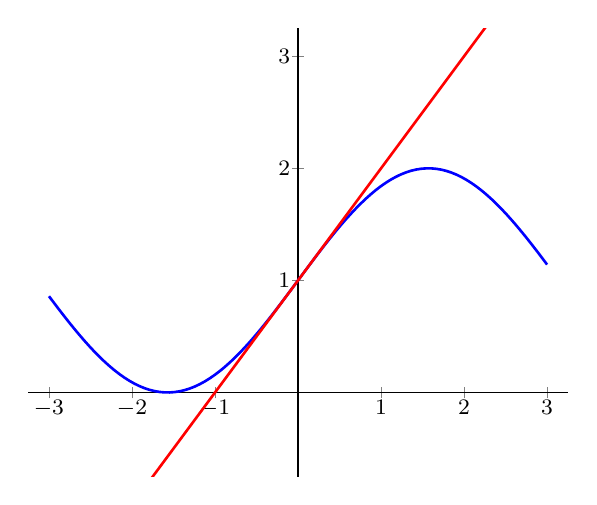
\begin{tikzpicture}
    \begin{axis}[
      grid style={line width=0.35pt, draw=gray!75},
      axis lines=center,
      axis line style={-},
      xmin=-3.25, xmax=3.25,
      ymin=-0.75, ymax=3.25,
      xtick={-6,-5,...,6},
      ytick={-6,-5,...,6},
      ticklabel style={font=\footnotesize,inner sep=0.5pt,fill=white,opacity=1.0, text opacity=1},
      every axis plot/.append style={line width=0.95pt, color=blue, samples=100}
      ]
      \addplot[-] expression[domain=-3:3]{1+sin(deg(x))};
      \addplot[-] expression[red]{x+1};
    \end{axis}
  \end{tikzpicture}
\end{flushright}
\begin{defn*}
  \textbf{Linear Approximation of $f$ at $a$.}
  
  Suppose $f$ if differentiable on an interval $I$ containing the point $a$. The \textbf{linear approximation} to $f$ at $a$ is the linear function.
  
  $$L(x)=f(a)+f'(a)(x-a),\ \textnormal{ for } x \textnormal{ in } I.$$
\end{defn*}
\pagebreak

\begin{ex*}
  Consider the function $f(x)=\dfrac{x}{x+1}$. Find the linearization at $a=1$. Use the linearization to estimate $f(1.1)$ and compare with the true value of $f(1.1)$.
\end{ex*}
\pagebreak

\begin{ex*}
  Find the linearization $L(x)$ of $f(x)=e^{3x-6}$ at $a=2$.
\end{ex*}
\vspace*{\stretch{1}}

\begin{ex*}
  Find the linearization $L(x)$ of $f(x)=9\parens{4x+11}^\frac{2}{3}$ at $a=4$.
\end{ex*}
\vspace*{\stretch{1}}

\begin{ex*}
  Find a linearization over an interval which will contain the given point $x_0$. Choose your center at a point \textit{near} $x_0$ but not at $x_0$ so that the given function and its derivative are easy to evaluate. Lastly, use the linearization to approximate $f(x_0)$.
\end{ex*}
\begin{enumerate}[label=\alph*), itemsep=\stretch{1}]
  \item $f(x)=x^2+2x,\ x_0=0.1$
  \item $f(x)=\sqrt[3]{x},\ x_0=8.5$.
\end{enumerate}
\vspace*{\stretch{1}}
\pagebreak

\begin{ex*}
  Use a linear approximation to estimate $\sqrt{146}$.
\end{ex*}
\vspace*{\stretch{1}}

\begin{ex*}
  Use a linear approximation to estimate $\parens{1.999}^4$.
\end{ex*}
\vspace*{\stretch{1}}

\begin{ex*}
  Use a linear approximation to estimate $\sqrt{\dfrac{5}{29}}$.
\end{ex*}
\vspace*{\stretch{1}}
\pagebreak

\begin{ex*}
  Find the linearization $L(x)$ of $f(x)=\sqrt{x^2+9}$ at $a=-4$. Use $L(x)$ to estimate $f(-4.1)$ and $\sqrt{23.44}$.
\end{ex*}
\vspace*{\stretch{1}}
\pagebreak

\begin{ex*}
  Use a linearization to show that $0.05$ is a good approximation for $\ln(1.05)$.
\end{ex*}
\pagebreak

\begin{ex*}
  Find the linearization of the following functions at the given point and use concavity to identify if the linearization is an overestimate or an underestimate.
\end{ex*}
\begin{enumerate}[label=\alph*),itemsep=\stretch{1}]
  \item $f(x)=\dfrac{2}{x};\, a=1$
  \item $f(x)=e\inv[x];\, a=\ln(2)$
\end{enumerate}
\vspace*{\stretch{1}}


\noindent
\fbox{\parbox{0.9875\linewidth}{
  \textbf{Summary: Uses of Linear Approximation}
  \begin{enumerate}
    \item 
      To approximate $f$ near $x=a$, use
        $$f(x)\approx L(x)=f(a)+f'(a)(x-a).$$
    \item 
      To approximate the change $\Delta y$ in the dependent variable when the independent variable $x$ changes from $a$ to $a+\Delta x$, use
        $$\Delta y\approx f'(a)\Delta x.$$
  \end{enumerate}
}}
\pagebreak

\begin{defn*}[Differentials]
  
  Let $f$ be differentiable on an interval containing $x$. A small change in $x$ is denoted by the \textbf{differential} $dx$. The corresponding change in $f$ is approximated by the \textbf{differential} $dy=f'(x)\,dx$. So if $\Delta x=dx$, where $\Delta x$ and $dx$ are both small, then $\Delta y\approx dy$:
    \[\Delta y= f(x+dx)-f(x)\approx dy=f'(x)\,dx.\]
    
\end{defn*}

\begin{ex*}
  Find the differential $dy$.
\end{ex*}
\begin{tasks}[after-item-skip=\stretch{1}, label=~](2)
  \task $y=\cos(x^2)$
  \task $y=\sqrt{1-x^2}$
  \task $y=4x^2-3x+2$
  \task $y=x\tan(x^3)$
  \task $y=\cos^5(x)$
  \task $f(x)=\sin\inv(x)$
\end{tasks}
\vspace*{\stretch{1}}
\pagebreak
\begin{ex*}
  Let $y=x^2$
\end{ex*}
\begin{enumerate}[label=\alph*), itemsep=\stretch{1}]
  \item Find $dy$
  \item If $x=1$ and $dx=0.01$, find $dy$.
  \item Compare $dy$ and $\Delta y$ at this point.
\end{enumerate}
\vspace*{\stretch{1}}

\begin{ex*}
  Let $y=\sqrt{3+x^2}$
\end{ex*}
\begin{enumerate}[label=\alph*), itemsep=\stretch{1}]
  \item Find $dy$
  \item If $x=1$ and $dx=-0.1$, find $dy$.
  \item Compare $dy$ and $\Delta y$ at this point.
\end{enumerate}
\vspace*{\stretch{1}}

\pagebreak
\begin{ex*}
  Suppose $f$ is differentiable on $(-\infty,\infty)$ and $f(5.01)-f(5)=0.25$. Use linear approximation to estimate the value of $f'(5)$.
\end{ex*}
\vspace*{\stretch{1}}

\begin{ex*}
  Suppose $f$ is differentiable on $(-\infty,\infty)$ and $f(5.99)=7$ and $f(6)=7.002$. Use linear approximation to estimate the value of $f'(6)$.
\end{ex*}
\vspace*{\stretch{1}}
\pagebreak

\begin{ex*}
  Compute $dy$ and $\Delta y$ for $y=e^x$ when $x=0$ and $\Delta x=0.5$.
\end{ex*}
\vspace*{\stretch{1}}

\begin{ex*}
  Approximate the change in the area of a circle when its radius increases from $2.00$ to $2.02\,m$.
\end{ex*}
\vspace*{\stretch{1}}

\begin{ex*}
  Approximate the change in the magnitude of the electrostatic force between two charges when the distance between them increases from $r=20\,m$ to $r=21\,m$ $(F(r)=0.01/r^2$).
\end{ex*}
\vspace*{\stretch{1}}
\pagebreak

\begin{ex*}
  Approximate the change in the volume of a right circular cylinder of fixed radius $r=20\,cm$ when its height decreases from $h=12\,cm$ to $h=11.9\,cm$ ($V(h)=\pi r^2h$).
\end{ex*}
\vspace*{\stretch{1}}

\begin{ex*}
  Approximate the change in the volume of a right circular cylinder of a right circular cone of fixed height $h=4\,m$ when its radius increases from $r=3\,m$ to $r=3.05\,m$ ($V(r)=\frac{1}{3}\pi r^2 h$).
\end{ex*}
\vspace*{\stretch{1}}
\pagebreak

\begin{ex*}
  The radius of a sphere is measured and found to be $0.7$ inches with a possible error in measurement of at most 0.01 inches.
\end{ex*}
\begin{enumerate}[label=\alph*), itemsep=\stretch{1}]
  \item What is the maximum error in using the value of the radius to compute the volume of the sphere?
  \item Find the relative error of the volume: \hfill\textit{relative error} $\dfrac{dV}{V}$\hspace*{50pt}
  
  What is the percentage error?
\end{enumerate}
\vspace*{\stretch{1}}
\pagebreak

\begin{ex*}
  The radius of a circular disk is given as $24\,cm$ with a maximum error in measurement of $0.2\,cm$.
\end{ex*}
\begin{enumerate}[label=\alph*), itemsep=\stretch{1}]
  \item Use differentials to estimate the maximum error in the calculated area of the disk.
  \item What is the relative error? What is the percentage error?
\end{enumerate}
\vspace*{\stretch{1}}
\pagebreak

\begin{ex*}
  Use differentials to estimate the amount of paint needed to apply a coat of paint $0.05\,cm$ thick to a hemispherical dome with diameter $50\,m$.
\end{ex*}
\vspace*{\stretch{1}}
\pagebreak
\end{document}

\input{briggs4_07}
\input{briggs4_05}
\input{briggs4_09}
\input{briggs5_01}
\input{briggs5_02}
\input{briggs5_03}
\documentclass[answers]{exam}
\usepackage{texPreamble}
\usepackage{relsize}
\usepackage{tabularx}
\extraheadheight{0.25in}
\extrafootheight{1.0in}
\extrawidth{1in}
% ----------------------------------------------------------------
\firstpagefootrule
\runningfootrule
\begin{document}
%\relscale{1.4}
\section{5.4: Working with Integrals}

\fbox{\parbox{0.9875\linewidth}{
  \textbf{Theorem 5.4: Integrals of Even and Odd Functions}
  
  Let $a$ be a positive real number and let $f$ be an integrable function on the interval $\sbrkt{-a,a}$.
  \begin{itemize}
    \item If $f$ is even, $\ds\int_{-a}^a f(x)\,dx=2\int_{0}^a f(x)\,dx.$
    \item If $f$ is odd, $\ds\int_{-a}^a f(x)\,dx=0.$
  \end{itemize}
}}

\begin{ex*}
  Rewrite the following trig functions to determine if it is even or odd:
  \begin{tasks}[label=\mbox{}](2)
    \task $\sin(-x)=$
    \task $\cos(-x)=$
    \task $\tan(-x)=$
    \task $\cot(-x)=$
    \task $\csc(-x)=$
    \task $\sec(-x)=$
  \end{tasks}
  Use this to rewrite and evaluate the following integrals:
\end{ex*}
\begin{tasks}[after-item-skip=\stretch{1}, label=\mbox{}](2)
  \task $\ds\int_{-\pi}^\pi \sin(x)\,dx$
  \task $\ds\int_{-\pi}^\pi \cos(x)\,dx$
  \task $\ds\int_{-\pi/4}^{\pi/4} \tan(x)\,dx$
  \task $\ds\int_{-\pi/4}^{\pi/4} \sec(x)\,dx$
\end{tasks}
\vspace*{\stretch{1}}
\textit{Note:} $\cot(x)$ and $\csc(x)$ are excluded here as they are not continuous on $\sbrkt{-\frac{\pi}{4},\frac{\pi}{4}}$.

\vspace*{-\baselineskip}
\pagebreak

\begin{ex*}
  Use symmetry to evaluate the following integrals:
\end{ex*}
\begin{tasks}[after-item-skip=\stretch{1}](1)
  \task $\ds\int_{-10}^{10} \frac{x}{\sqrt{200-x^2}}\,dx$
  \task $\ds\int_{-2}^{2}\parens{x^9-3x^5+2x^2-10}\,dx$
\end{tasks}
\vspace*{\stretch{1}}
\pagebreak

\begin{tasks}[after-item-skip=\stretch{1}, resume](1)
  \task $\ds\int_{-\frac{\pi}{4}}^{\frac{\pi}{4}}\sin^5(x)\,dx$
  \task $\ds\int_{-1}^{1}\parens{1-\abs{x}}\,dx$
  \task $\ds\int_{-2}^{2}\frac{x^3-4x}{x^2+1}\,dx$
\end{tasks}
\vspace*{\stretch{1}}
\pagebreak

\begin{ex*}
  Given that $f(x)$ is even and $\ds\int_{-8}^{8} f(x)\,dx=18$, find
\end{ex*}
\begin{tasks}(2)
  \task $\ds\int_{0}^{8}f(x)\,dx$
  \task $\ds\int_{-8}^{8}xf(x)\,dx$
\end{tasks}
\vspace*{\stretch{1}}
\begin{ex*}
  Given that $f(x)$ is odd and $\ds\int_{0}^{4} f(x)\,dx=3$ and $\ds\int_0^8 f(x)\,dx=9$, find
\end{ex*}
\begin{tasks}(2)
  \task $\ds\int_{-4}^{8}f(x)\,dx$
  \task $\ds\int_{-8}^{4}f(x)\,dx$
\end{tasks}
\vspace*{\stretch{1}}
\pagebreak

\begin{ex*}
  Use symmetry to explain why
\end{ex*}
  \[\int_{-4}^{4}\parens{5x^4+3x^3+2x^2+x+1}\,dx=2\int_0^4 \parens{5x^4+2x^2+1}\,dx\]

  \vspace*{\stretch{1}}
\begin{ex*}
  Evaluate
\end{ex*}
  $\ds\int_{-\frac{\pi}{2}}^{\frac{\pi}{2}}\parens{\cos(2\theta)+\cos(\theta)\sin(\theta)-3\sin(\theta^5)}\,d\theta$
\vspace*{\stretch{1}}
\begin{ex*}
  While the following integrals are not on symmetric intervals, symmetry still applies here:
\end{ex*}
\begin{tasks}(3)
  \task $\ds\int_0^\pi \cos(x)\,dx$
  \task $\ds\int_0^{2\pi} \sin(x)\,dx$
  \task $\ds\int_0^{4\pi} \cos(x)\,dx$
\end{tasks}
\vspace*{\stretch{1}}
\pagebreak

\begin{defn*}[Average Value of a Function]
  The average value of an integrable function $f$ on the interval $\sbrkt{a,b}$ is
    \[\bar f= \frac{1}{b-a}\int_a^b f(x)\,dx.\]
\end{defn*}
\begin{ex*}
  Find the average value of $f(x)=-\dfrac{x^2}{2}$ on $\sbrkt{0,3}$.
\end{ex*}
\vspace*{\stretch{1}}
\begin{ex*}
  Find the average value of $f(x)=3x^2-3$ on $\sbrkt{0,1}$.
\end{ex*}
\vspace*{\stretch{1}}
\begin{ex*}
  Find the average value of $f(t)=t^2-t$ on $\sbrkt{-2,1}$.
\end{ex*}
\vspace*{\stretch{1}}
\pagebreak

\begin{ex*}
  Find the average value of $f(x)=\dfrac{1}{x^2+1}$ on $\sbrkt{-1,1}$.
\end{ex*}
\vspace*{\stretch{1}}
\begin{ex*}
  Find the average value of $f(x)=\dfrac{1}{x}$ on $\sbrkt{1,e}$.
\end{ex*}
\vspace*{\stretch{1}}
\begin{ex*}
  Find the average value of $f(x)=x^\frac{1}{n}$ on $\sbrkt{0,1}$.
\end{ex*}
\vspace*{\stretch{1}}
\pagebreak

\begin{ex*}
  The velocity in $m/s$ of an object moving along a line over the time interval $\sbrkt{0,6}$ is $v(t)=t^2+3t$. Find the average velocity of the object over this time interval.
\end{ex*}
\vspace*{\stretch{1}}

\begin{ex*}
  A rock is launched vertically upward from the ground with a speed of $64 ft/s$. The height of the rock (in $ft$) above the ground after $t$ seconds is given by the function $s(t)=-16t^2+64t$. Find its average velocity during its flight.
\end{ex*}
\vspace*{\stretch{1}}

\pagebreak
\begin{ex*}
  The surface of a water wave is described by $y=5\parens{1+\cos(x)}$, for $-\pi\leq x\leq \pi$, where $y=0$ corresponds to a trough of the wave. Find the average height of the wave above the trough on $\sbrkt{-\pi,\pi}$.
\end{ex*}

\noindent
\begin{minipage}{0.5\linewidth}
  \begin{tikzpicture}
    \begin{axis}[
      axis lines=center,
      axis line style={->},
      xmin=-1.2*pi, xmax=1.2*pi,
      ymin=-0.5, ymax=11,
      height=2.5in, width=3.5in,
      xtick={-3.141592654,-1.570796327,1.570796327,3.141592654},
      xticklabels={$-\pi$,$-\sfrac{\pi}{2}$,$\sfrac{\pi}{2}$,$\pi$},
      ticklabel style={font=\small,inner sep=0.5pt,fill=white,opacity=1.0, text opacity=1},
      xlabel=$x$, xlabel style={at={(ticklabel* cs:1)},anchor=north west},
      ylabel=$y$, ylabel style={at={(ticklabel* cs:1)},anchor=south west},
      every axis plot/.append style={line width=0.95pt, color=blue, samples=100}
      ]
      \addplot[-] expression[domain=-pi:pi] {5*(1+cos(x*180/pi))};
    \end{axis}
  \end{tikzpicture}
\end{minipage}
\pagebreak

\noindent
\fbox{\parbox{0.9875\linewidth}{
  \textbf{Theorem 5.5: Mean Value Theorem for Integrals}

  Let $f$ be continuous on the interval $\sbrkt{a,b}$. There exists a point $c$ in $\parens{a,b}$ such that 
    \[f(c)=\bar f=\frac{1}{b-a}\int_a^b f(t)\,dt\]
}}
\begin{ex*}
  For the following problems, find the point(s) that satisfy the Mean Value Theorem for Integrals.
\end{ex*}
\begin{tasks}[after-item-skip=\stretch{1}](1)
  \task $f(x)=\dfrac{1}{x^2}$ on $\sbrkt{1,4}$.
  \task $f(x)=e^x$ on $\sbrkt{0,2}$.
  \task $f(x)=\cos(x)$ on $\sbrkt{-\dfrac{\pi}{2},\dfrac{\pi}{2}}$
  \task $f(x)=1-\abs{x}$ on $\sbrkt{-1,1}$.
\end{tasks}
\vspace*{\stretch{1}}

%TODO remove relscale
\pagebreak
\end{document}

\input{briggs5_05}
\end{document}
